\startappendix{Additional Information}
\label{chapter:appendix}

\begin{figure}[h]
\centering
\includegraphics[width=16cm, height=8cm]{Figures/ROI_score}
\caption{BrainBench 2 vs. 2 accuracies across all 43 anatomical brain regions.}
\label{all43}
\end{figure}
\newpage


\begin{figure*}[!hb]
    \centering
    \begin{subfigure}[t]{0.49\textwidth}
        \includegraphics[width=\textwidth]{Figures/InceptionOrg}
        \caption{The original inception module \\from \textit{GoogLeNet}.}
    \end{subfigure}%
    \centering
    \begin{subfigure}[t]{0.49\textwidth}
        \includegraphics[width=\textwidth]{Figures/InceptionV2}
        \centering
        \caption{$5*5$ convolutions broken down into two $3*3$ convolutions. This inception module would be referred to as \textit{Type A}.}
        \label{typea}
    \end{subfigure}
        \centering
    \begin{subfigure}[t]{0.49\textwidth}
        \includegraphics[width=7cm]{Figures/typeb}
        \caption{An $n*n$ convolution is completely \\factorized into $1*n$ and $n*1$ \\convolutions(here n=7). This inception \\module would be referred to as \textit{Type B}. }
        \label{typeb}
    \end{subfigure}
    \centering
        \begin{subfigure}[t]{0.49\textwidth}
        \includegraphics[width=10cm]{Figures/InceptionV2b}
        \caption{Intermediate factorization of the inception module for extracting high dimensional representations.This inception module would be referred to as \textit{Type C}.}
    \label{typec}
    \end{subfigure}
    \caption{Factorizations into smaller convolutions in Inception-v3}  
    \label{Inceptiontypes}
    This figure summarizes the changes in the inception module from the original GoogLeNet. Here factorization of convolutional layers are done to make the computational cost cheaper. The diagrams above are extracted from the original paper by Szegedy et al.~\cite{Inception-v3}.
\end{figure*}



\newpage
\begin{figure}[!hb]
\centering
\includegraphics[width=10cm, height=20cm]{Figures/vggnewarch}
\caption{2 vs. 2 accuracy through architecture diagram of VGG16}
\label{VGGARCH}
The architecture diagram of VGG16 is annotated with 2 vs. 2 accuracy of layers against Skip-gram word-vectors~\cite{VGG16}. This is a high resolution image and could be zoomed and viewed in a pdf.
\end{figure}


\newpage
\begin{figure}[!hb]
\centering
\includegraphics[width=10cm, height=20cm]{Figures/resnetnewarch}
\caption{2 vs. 2 accuracy through architecture diagram of ResNet50}
\label{RESARCH}
The architecture diagram of ResNet50 is annotated with 2 vs. 2 accuracy of layers against Skip-gram word-vectors~\cite{ResNet}. This is a high resolution image and could be zoomed and viewed in a pdf.
\end{figure}


\newpage
\begin{figure}[!hb]
\centering
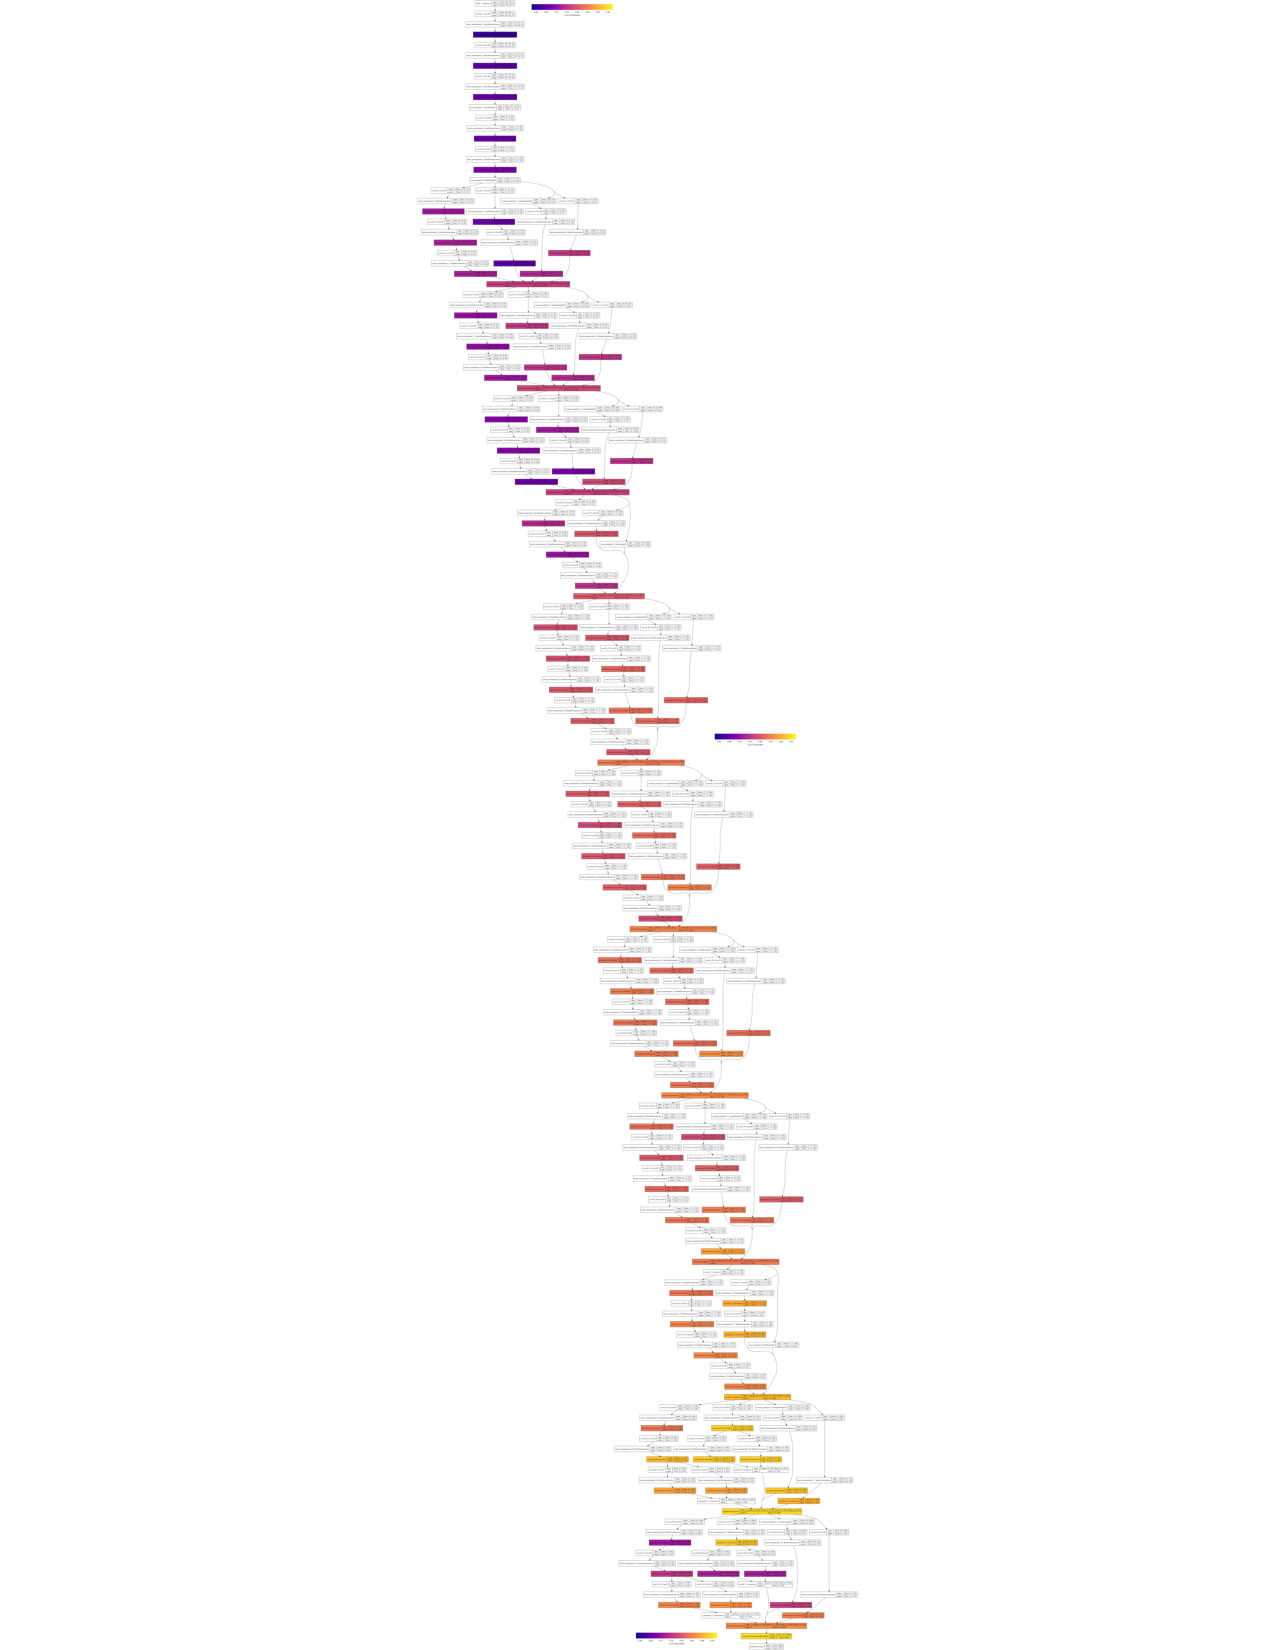
\includegraphics[width=10cm, height=20cm]{Figures/inceptionnewarch}
\caption{2 vs. 2 accuracy through architecture diagram of Inception-v3}
\label{INCARCH}
The architecture diagram of Inception-v3 is annotated with 2 vs. 2 accuracy of layers against Skip-gram word-vectors~\cite{Inception-v3}. This is a high resolution image and could be zoomed and viewed in a pdf.
\end{figure}






